\section{Phân tích \& Thiết kế hệ thống}

\subsection{Kiến trúc hệ thống}
\indent \indent Hệ thống MyTicket được xây dựng theo mô hình client–server monolith gồm frontend React SPA, backend Node.js Express và cơ sở dữ liệu MongoDB Atlas, đồng thời tích hợp nhiều dịch vụ ngoài phục vụ thanh toán, email, AI chatbot và recommendation.\\
\indent Kiến trúc được tổ chức thành các lớp chính gồm:
\begin{itemize}
    \item[1.] Lớp người dùng và giao diện frontend.
    \item[2.] Lớp backend xử lý nghiệp vụ.
    \item[3.] Lớp cơ sở dữ liệu trung tâm.
    \item[4.] Lớp tích hợp dịch vụ bên ngoài.
    \item[5.] Lớp tác vụ nền và pipeline AI recommendation.
\end{itemize}
Khác với kiến trúc microservice, toàn bộ nghiệp vụ chính của hệ thống hiện tại được xử lý trong một backend Express duy nhất, giúp đồng bộ dữ liệu, dễ triển khai và thuận tiện cho bảo trì trong phạm vi đồ án tốt nghiệp.
\begin{figure}[H]
    \centering
    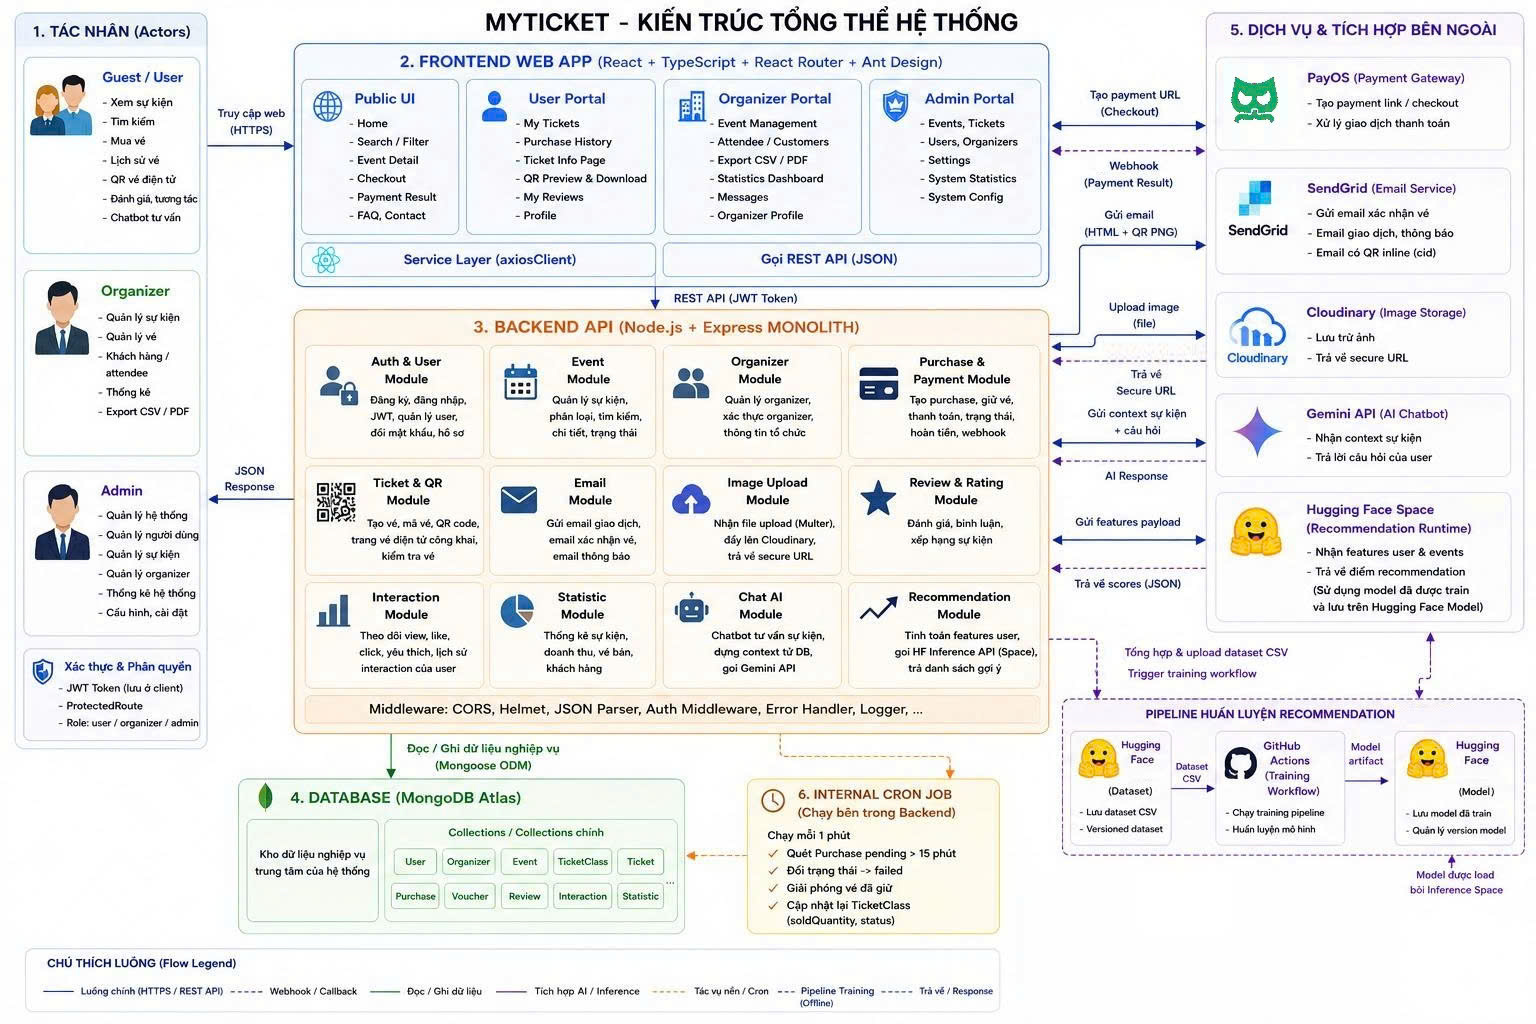
\includegraphics[width=1\textwidth]{Images/kiến trúc toàn hệ thống.jpg}
    \vspace{10pt}
    \caption{Kiến trúc hệ thống}
    \label{fig:hdfs_architecture}
\end{figure}
\begin{itemize}
    \item[1.] \textbf{Client Side – Frontend Web App}\\
    Người dùng truy cập hệ thống thông qua trình duyệt web với các nhóm vai trò: khách hàng, ban tổ chức và quản trị viên.\\
    Frontend được phát triển bằng React + TypeScript + React Router + Ant Design theo mô hình SPA (Single Page Application).\\
    Frontend chịu trách nhiệm:
    \begin{itemize}
        \item[-] Hiển thị giao diện tìm kiếm và mua vé.
        \item[-] Hiển thị lịch sử vé, QR code và vé điện tử.
        \item[-] Cung cấp giao diện quản lý sự kiện cho organizer và admin.
        \item[-] Gọi REST API tới backend thông qua axiosClient.
        \item[-] Lưu JWT token và kiểm soát truy cập bằng ProtectedRoute.
    \end{itemize}
    Các vùng chức năng chính trên frontend gồm:
    \begin{itemize}
        \item[-] Public UI.
        \item[-] User Portal.
        \item[-] Organizer Portal.
        \item[-] Admin Portal.
    \end{itemize}
    Frontend trong môi trường production được triển khai độc lập với backend và giao tiếp thông qua HTTPS REST API.
    \item[2.] \textbf{Server Side – Backend API}: \\
    Các chức năng chính của backend bao gồm:
    \begin{itemize}
        \item[-] Xác thực và phân quyền bằng JWT.
        \item[-] Quản lý user, organizer, event, ticket, purchase;
        \item[-] Xử lý checkout và thanh toán;
        \item[-] Phát hành vé điện tử và QR code;
        \item[-] Gửi email xác nhận;
        \item[-] Upload ảnh;
        \item[-] Chatbot AI;
        \item[-] Recommendation;
        \item[-] Thống kê và tracking interaction.
    \end{itemize}
    Các module nghiệp vụ chính trong backend gồm:
    \begin{table}[H]
    \centering
    \caption{Danh sách các module nghiệp vụ trong backend}
    \begin{tabular}{|c|l|}
    \hline
    \textbf{STT} & \textbf{Module} \\ \hline
    1 & Auth \& User Module \\ \hline
    2 & Event Module \\ \hline
    3 & Organizer Module \\ \hline
    4 & Purchase \& Payment Module \\ \hline
    5 & Ticket \& QR Module \\ \hline
    6 & Email Module \\ \hline
    7 & Image Upload Module \\ \hline
    8 & Review \& Rating Module \\ \hline
    9 & Statistic Module \\ \hline
    10 & Chat AI Module \\ \hline
    11 & Recommendation Module \\ \hline
    \end{tabular}
    \end{table}
    Backend giao tiếp với frontend bằng REST API và trả dữ liệu ở định dạng JSON.
    \item[3.] \textbf{ Database Layer – MongoDB Atlas}\\
    Hệ thống sử dụng MongoDB Atlas làm cơ sở dữ liệu trung tâm.
    MongoDB lưu trữ toàn bộ dữ liệu nghiệp vụ như:
    \begin{table}[H]
    \centering
    \caption{Danh sách các collection trong MongoDB}
    \begin{tabular}{|c|c|}
    \hline
    \textbf{STT} & \textbf{Collection} \\ \hline
    1 & User \\ \hline
    2 & Organizer \\ \hline
    3 & Event \\ \hline
    4 & TicketClass \\ \hline
    5 & Ticket \\ \hline
    6 & Purchase \\ \hline
    7 & Voucher \\ \hline
    8 & Review \\ \hline
    9 & Interaction \\ \hline
    10 & Statistic \\ \hline
    \end{tabular}
    \end{table}
    Backend sử dụng Mongoose ODM để định nghĩa schema, validation và truy vấn dữ liệu.\\
    Mọi thao tác đọc/ghi dữ liệu đều được thực hiện thông qua backend nhằm đảm bảo tính bảo mật và toàn vẹn dữ liệu.
    \item[4.] \textbf{Tích hợp dịch vụ bên ngoài}\\
    Hệ thống tích hợp nhiều dịch vụ ngoài nhằm mở rộng chức năng thực tế:
    \begin{itemize}
        \item[-] \textbf{PayOS – Thanh toán trực tuyến}\\
        Backend tạo payment URL thông qua API của PayOS. Sau khi người dùng thanh toán thành công, PayOS gửi webhook về backend để cập nhật trạng thái giao dịch và phát hành vé điện tử.
        \item[-] \textbf{SendGrid – Gửi email giao dịch}\\
        Hệ thống sử dụng SendGrid để gửi email xác nhận đặt vé, email thông báo và email chứa QR code vé điện tử.
        \item[-] \textbf{Cloudinary – Lưu trữ ảnh}\\
        Frontend upload ảnh tới backend, sau đó backend gửi ảnh lên Cloudinary và nhận về secure URL để lưu vào hệ thống.
        \item[-] \textbf{Gemini API – Chatbot AI}\\
        Backend lấy dữ liệu sự kiện từ MongoDB, xây dựng context rồi gửi tới Gemini API để tạo phản hồi chatbot tư vấn sự kiện cho người dùng.
        \item[-] \textbf{Hugging Face – Recommendation System}\\
        Hệ thống recommendation được triển khai theo hai phần:
        \begin{itemize}
            \item[+] runtime inference thông qua Hugging Face Space API.
            \item[+] pipeline huấn luyện mô hình thông qua Hugging Face Hub (Dataset + Model) và GitHub Actions.
        \end{itemize}
        Backend gửi feature payload của user và event tới Hugging Face Space để nhận recommendation score và trả kết quả gợi ý cho frontend.\\
        Sau khi pipeline training hoàn tất, mô hình được lưu lên Hugging Face Model và được Hugging Face Space sử dụng lại cho quá trình inference recommendation runtime.
    \end{itemize}
    \item[5.] \textbf{Internal Cron Job – Tác vụ nền}\\
    Hệ thống sử dụng node-cron chạy trực tiếp bên trong backend process để xử lý các tác vụ định kỳ.\\
    Cron job hiện tại thực hiện:
    \begin{itemize}
        \item[-] Quét các đơn hàng pending quá thời gian quy định.
        \item[-] Chuyển trạng thái purchase sang failed;
        \item[-] Giải phóng vé giữ chỗ;
        \item[-] Cập nhật lại số lượng vé đã bán và trạng thái TicketClass.
    \end{itemize}
    \item[6.] \textbf{Ưu điểm của kiến trúc hiện tại}
    \begin{itemize}
        \item[-] Kiến trúc rõ ràng, dễ triển khai và phù hợp với mô hình full-stack web application.
        \item[-] Backend monolith giúp đồng bộ dữ liệu và giảm độ phức tạp triển khai.
        \item[-] Dễ tích hợp các dịch vụ thực tế như PayOS, SendGrid, Cloudinary và AI services.
        \item[-] Hỗ trợ recommendation và chatbot AI nhằm tăng khả năng cá nhân hóa trải nghiệm người dùng.
        \item[-] Hệ thống QR vé điện tử và email giao dịch giúp tăng tính thực tiễn của ứng dụng.
        \item[-] Dễ mở rộng thêm module mới trong tương lai mà không ảnh hưởng lớn tới kiến trúc hiện tại.
    \end{itemize}
\end{itemize}

\subsection{Thiết kế Database}

\subsubsection{Tổng quan cơ sở dữ liệu}
Hệ thống MyTicket sử dụng MongoDB làm hệ quản trị cơ sở dữ liệu chính nhằm hỗ trợ lưu trữ dữ liệu phi cấu trúc và khả năng mở rộng linh hoạt cho hệ thống bán vé sự kiện trực tuyến.\\
Mô hình dữ liệu được thiết kế theo hướng document-oriented, trong đó mỗi thực thể được biểu diễn dưới dạng một collection riêng biệt. Các collections được liên kết với nhau thông qua ObjectId references nhằm đảm bảo khả năng mở rộng, giảm dư thừa dữ liệu và tối ưu hiệu năng truy vấn.
\begin{figure}[H]
    \centering
    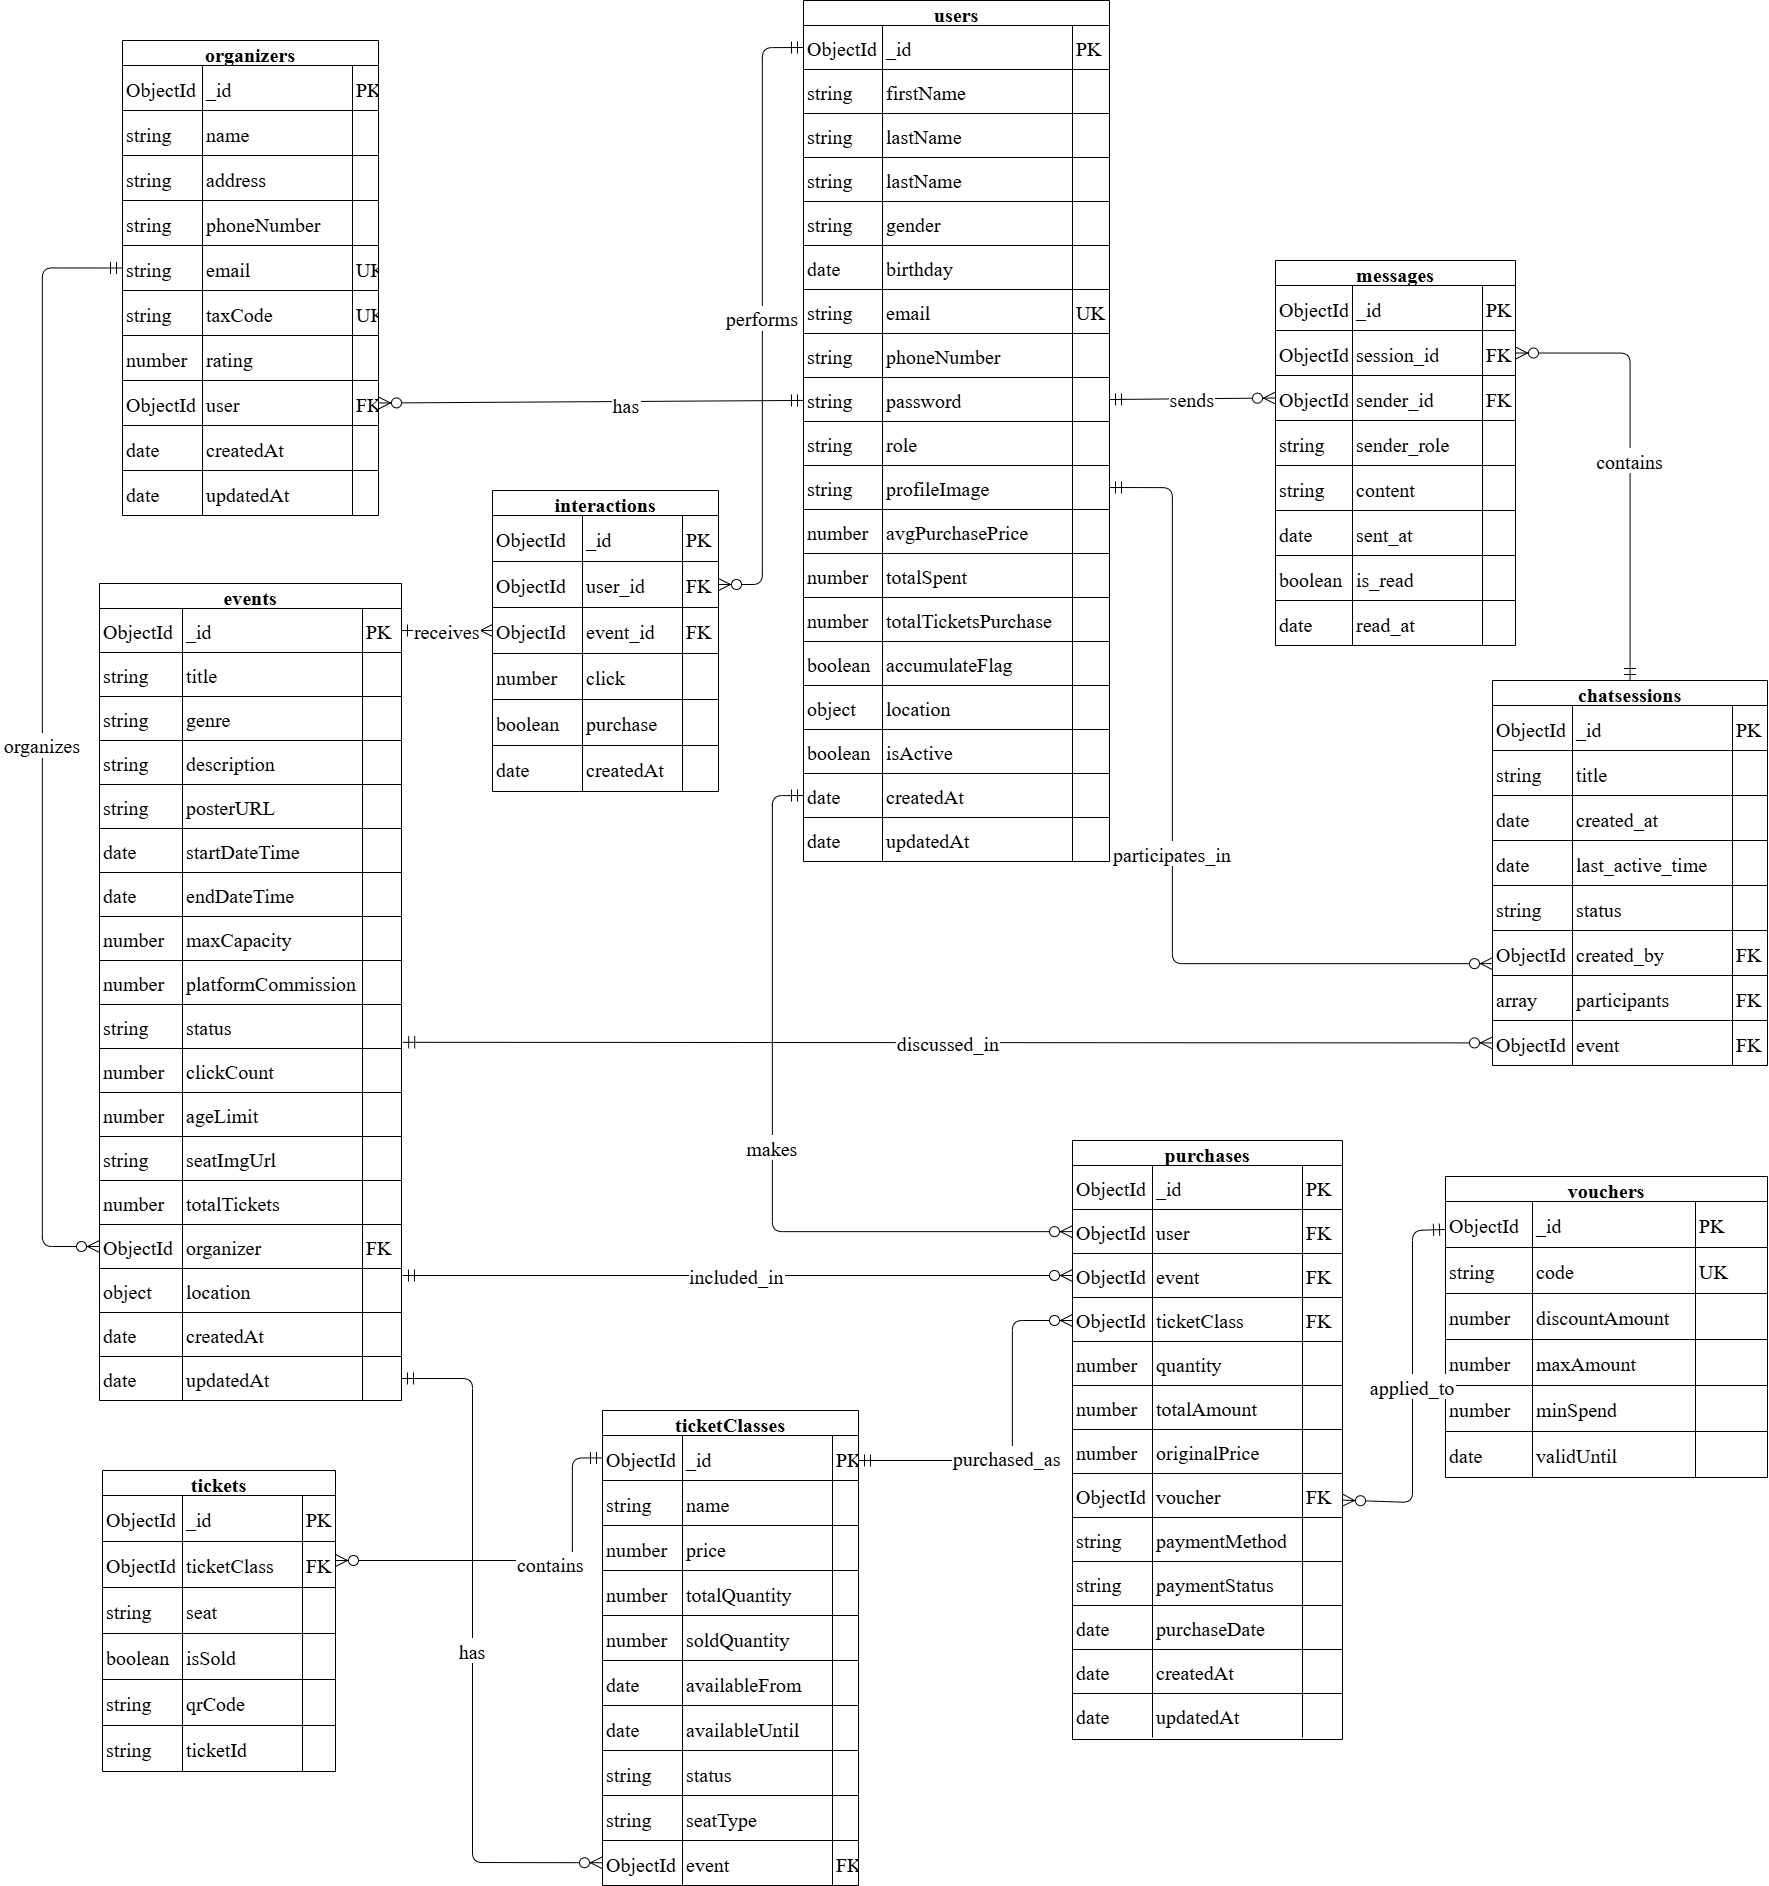
\includegraphics[width=1\textwidth]{Images/schema.png}
    \vspace{15pt}
    \caption{MongoDB Data Model Diagram}
\end{figure}
Cơ sở dữ liệu của hệ thống bao gồm các collection chính:
\begin{itemize}
    \item[1.] users
    \item[2.] organizers
    \item[3.] events
    \item[4.] ticketClasses
    \item[5.] tickets
    \item[6.] purchases
    \item[7.] vouchers
    \item[8.] reviews
    \item[9.] interactions
\end{itemize}
Hệ thống sử dụng mô hình reference thay vì embedding đối với các thực thể có kích thước lớn hoặc tần suất cập nhật cao như events, purchases và tickets nhằm:
\begin{itemize}
    \item[-] Giảm trùng lặp dữ liệu.
    \item[-] Tăng khả năng mở rộng hệ thống.
    \item[-] Tối ưu hiệu suất cập nhật dữ liệu.
\end{itemize}

\subsubsection{Mô hình quan hệ dữ liệu}
Trong hệ thống, collection users đóng vai trò trung tâm và liên kết với nhiều collection khác như purchases, reviews, interactions và organizers.\\
Một organizer được ánh xạ với một tài khoản người dùng nhằm hỗ trợ cơ chế phân quyền giữa người tham gia và nhà tổ chức sự kiện.\\
Mỗi event thuộc về một organizer và có thể chứa nhiều ticket classes nhằm hỗ trợ nhiều loại vé khác nhau như VIP, Standard hoặc Early Bird.\\
Khi người dùng thực hiện giao dịch mua vé, hệ thống tạo purchase record đồng thời sinh ra các ticket tương ứng để phục vụ check-in và xác thực vé.\\
Ngoài ra, hệ thống còn hỗ trợ:
\begin{itemize}
    \item[-] Voucher giảm giá.
    \item[-] Đánh giá sự kiện.
    \item[-] Tracking hành vi người dùng thông qua interactions.
\end{itemize}

\subsubsection{Chi tiết các collection hệ thống}

\textbf{a. Collection users} \\
Collection users lưu trữ thông tin tài khoản của người dùng trong hệ thống.\\
Các thực thể này gồm có các thuộc tính:
\setlength{\LTleft}{0pt}
\setlength{\LTright}{0pt}
\begin{longtable}{|p{4cm}|p{11.2cm}|}
\caption{Cấu trúc dữ liệu của bảng Users}\\[15pt]
\hline
\textbf{Field} & \textbf{Description} \\ \hline
\_id & ObjectId - Định danh duy nhất của người dùng \\ \hline
firstName & String - Tên người dùng \\ \hline
lastName & String - Họ người dùng \\ \hline
email & String - Email đăng nhập \\ \hline
password & String - Mật khẩu đã được hash \\ \hline
phoneNumber & String - Số điện thoại \\ \hline
birthday & Date - Ngày sinh \\ \hline
gender & String - Giới tính \\ \hline
profileImage & String - Ảnh đại diện \\ \hline
role & String - Vai trò người dùng \\ \hline
totalSpent & Decimal - Tổng chi tiêu \\ \hline
totalTicketsPurchased & Int - Tổng số vé đã mua \\ \hline
avgPurchasePrice & Decimal - Giá trị mua trung bình \\ \hline
isActive & Boolean - Trạng thái tài khoản \\ \hline
location & Object - Thông tin vị trí người dùng \\ \hline
OTP\_CODE & Object - Thông tin OTP xác thực \\ \hline
createdAt & Date - Thời gian tạo \\ \hline
updatedAt & Date - Thời gian cập nhật \\ \hline
\end{longtable}
\textbf{Quan hệ dữ liệu:}
\begin{itemize}
    \item[-] Một user có thể tạo nhiều purchase.
    \item[-] Một user có thể thực hiện nhiều review.
    \item[-] Một user có thể tương tác với nhiều event.
\end{itemize}

\textbf{b. Collection organizers} \\
Collection organizers lưu trữ thông tin của các nhà tổ chức sự kiện trên nền tảng
\setlength{\LTleft}{0pt}
\setlength{\LTright}{0pt}
\begin{longtable}{|p{4cm}|p{11.2cm}|}
\caption{Các thuộc tính của bảng Organizers}\\[15pt]
\hline
\textbf{Field} & \textbf{Description} \\ \hline
\_id & ObjectId - Định danh organizer \\ \hline
user & ObjectId - Tham chiếu đến user \\ \hline
name & String - Tên organizer \\ \hline
email & String - Email liên hệ \\ \hline
phoneNumber & String - Số điện thoại \\ \hline
address & String - Địa chỉ \\ \hline
taxCode & String - Mã số thuế \\ \hline
rating & Decimal - Điểm đánh giá \\ \hline
createdAt & Date - Thời gian tạo \\ \hline
updatedAt & Date - Thời gian cập nhật \\ \hline
\end{longtable}
\textbf{Quan hệ dữ liệu:}
\begin{itemize}
    \item[-] Một organizer thuộc về một user.
    \item[-] Một organizer có thể tạo nhiều event.
    \item[-] Một organizer có thể nhận nhiều review.
\end{itemize}
\textbf{Quyết định thiết kế:} Collection organizers được tách riêng khỏi users nhằm hỗ trợ
\begin{itemize}
    \item[-] Phân quyền rõ ràng.
    \item[-] Mở rộng chức năng quản lý organizer.
    \item[-] Quản lý thống kê và doanh thu riêng.
\end{itemize}

\textbf{c. Collection events}\\
Collection events lưu trữ thông tin các sự kiện được tạo bởi organizer trên hệ thống.\\
Đây là collection trung tâm của hệ thống và liên kết với nhiều collection khác như ticketClasses, reviews, interactions và purchases.
\setlength{\LTleft}{0pt}
\setlength{\LTright}{0pt}
\begin{longtable}{|p{4cm}|p{11.2cm}|}
\caption{Các thuộc tính của bảng Events}\\[15pt]
\hline
\textbf{Field} & \textbf{Description} \\ \hline
\_id & ObjectId - Định danh duy nhất của sự kiện \\ \hline
title & String - Tên sự kiện \\ \hline
genre & String - Thể loại sự kiện \\ \hline
description & String - Mô tả sự kiện \\ \hline
startDateTime & Date - Thời gian bắt đầu \\ \hline
endDateTime & Date - Thời gian kết thúc \\ \hline
maxCapacity & Int - Sức chứa tối đa \\ \hline
totalTickets & Int - Tổng số vé \\ \hline
clickCount & Int - Số lượt truy cập \\ \hline
ageLimit & Int - Giới hạn độ tuổi \\ \hline
platformCommission & Int - Phí hoa hồng nền tảng \\ \hline
status & String - Trạng thái sự kiện \\ \hline
posterURL & String - Đường dẫn poster \\ \hline
seatImgUrl & String - Hình sơ đồ ghế \\ \hline
organizer & ObjectId - Organizer sở hữu \\ \hline
location & Object - Thông tin địa điểm \\ \hline
createdAt & Date - Thời gian tạo \\ \hline
updatedAt & Date - Thời gian cập nhật \\ \hline
\end{longtable}
\textbf{Quan hệ dữ liệu:}
\begin{itemize}
    \item[-] Một organizer có thể tạo nhiều event.
    \item[-] Một event có thể có nhiều ticketClasses.
    \item[-] Một event có thể nhận nhiều reviews.
    \item[-] Một event có thể phát sinh nhiều purchases.
    \item[-] Một event có thể có nhiều interactions.
\end{itemize}
\textbf{Quyết định thiết kế:} Collection events sử dụng reference đến organizers thay vì embedding nhằm
\begin{itemize}
    \item[-] Tránh dư thừa dữ liệu organizer.
    \item[-] Dễ dàng cập nhật thông tin organizer.
    \item[-] Tăng khả năng mở rộng hệ thống.
\end{itemize}

\textbf{d. Collection ticketClasses}\\
Collection ticketClasses lưu trữ thông tin các loại vé thuộc từng sự kiện.
\setlength{\LTleft}{0pt}
\setlength{\LTright}{0pt}
\begin{longtable}{|p{4cm}|p{11.2cm}|}
\caption{Các thuộc tính của bảng TicketClasses}\\[15pt]
\hline
\textbf{Field} & \textbf{Description} \\ \hline
\_id & ObjectId - Định danh loại vé \\ \hline
event & ObjectId - Sự kiện tương ứng \\ \hline
name & String - Tên loại vé \\ \hline
seatType & String - Loại chỗ ngồi \\ \hline
price & Decimal - Giá vé \\ \hline
totalQuantity & Int - Tổng số lượng vé \\ \hline
soldQuantity & Int - Số lượng đã bán \\ \hline
availableFrom & Date - Thời gian mở bán \\ \hline
availableUntil & Date - Thời gian kết thúc bán \\ \hline
status & String - Trạng thái vé \\ \hline
\end{longtable}
\textbf{Quan hệ dữ liệu:}
\begin{itemize}
    \item[-] Một event có nhiều ticketClasses.
    \item[-] Một ticketClass có thể xuất hiện trong nhiều purchases.
    \item[-] Một ticketClass có thể sinh ra nhiều tickets.
\end{itemize}

\textbf{e. Collection tickets}\\
Collection tickets lưu trữ thông tin từng vé riêng lẻ được sinh ra sau khi người dùng hoàn tất giao dịch mua vé.
\setlength{\LTleft}{0pt}
\setlength{\LTright}{0pt}
\begin{longtable}{|p{4cm}|p{11.2cm}|}
\caption{Các thuộc tính của bảng Tickets}\\[15pt]
\hline
\textbf{Field} & \textbf{Description} \\ \hline
\_id & ObjectId - Định danh vé \\ \hline
ticketId & String - Mã vé \\ \hline
seat & String - Vị trí ghế \\ \hline
isSold & Boolean - Trạng thái bán \\ \hline
purchase & ObjectId - Giao dịch mua vé \\ \hline
ticketClass & ObjectId - Loại vé \\ \hline
\end{longtable}
\textbf{Quan hệ dữ liệu:}
\begin{itemize}
    \item[-] Một purchase có thể chứa nhiều tickets.
    \item[-] Một ticket thuộc về một ticketClass.
\end{itemize}
\textbf{Quyết định thiết kế:} Collection tickets được tách riêng khỏi purchases nhằm
\begin{itemize}
    \item[-] Quản lý từng vé độc lập.
    \item[-] Hỗ trợ xác thực check-in.
    \item[-] Chống gian lận vé.
    \item[-] Mở rộng cho QR validation trong tương lai.
\end{itemize}

\textbf{f. Collection purchases}\\
Collection purchases lưu trữ thông tin giao dịch mua vé của người dùng.
Mỗi document đại diện cho một giao dịch thanh toán hoàn chỉnh trong hệ thống.
\setlength{\LTleft}{0pt}
\setlength{\LTright}{0pt}
\begin{longtable}{|p{4cm}|p{11.2cm}|}
\caption{Các thuộc tính của bảng Purchases}\\[15pt]
\hline
\textbf{Field} & \textbf{Description} \\ \hline
\_id & ObjectId - Định danh giao dịch \\ \hline
user & ObjectId - Người thực hiện giao dịch \\ \hline
event & ObjectId - Sự kiện được mua vé \\ \hline
ticketClass & ObjectId - Loại vé \\ \hline
voucher & ObjectId - Voucher áp dụng \\ \hline
quantity & Int - Số lượng vé \\ \hline
originalPrice & Decimal - Giá gốc \\ \hline
totalAmount & Int - Tổng thanh toán \\ \hline
paymentMethod & String - Phương thức thanh toán \\ \hline
paymentStatus & String - Trạng thái thanh toán \\ \hline
orderCode & Int - Mã đơn hàng \\ \hline
purchaseDate & Date - Thời gian mua \\ \hline
createdAt & Date - Thời gian tạo \\ \hline
updatedAt & Date - Thời gian cập nhật \\ \hline
\end{longtable}
\textbf{Quan hệ dữ liệu:}
\begin{itemize}
    \item[-] Một user có thể có nhiều purchase.
    \item[-] Một purchase thuộc về một event.
    \item[-] Một purchase có thể sinh ra nhiều tickets.
    \item[-] Một purchase có thể áp dụng voucher.
\end{itemize}
\textbf{Quyết định thiết kế:} Collection purchases được thiết kế riêng nhằm
\begin{itemize}
    \item[-] Quản lý transaction hiệu quả.
    \item[-] Hỗ trợ rollback/payment verification.
    \item[-] Tối ưu việc thống kê doanh thu.
\end{itemize}

\textbf{g. Collection vouchers}\\
Collection vouchers lưu trữ thông tin mã giảm giá được sử dụng trong hệ thống.
\setlength{\LTleft}{0pt}
\setlength{\LTright}{0pt}
\begin{longtable}{|p{4cm}|p{11.2cm}|}
\caption{Các thuộc tính của bảng Vouchers}\\[15pt]
\hline
\textbf{Field} & \textbf{Description} \\ \hline
\_id & ObjectId - Định danh voucher \\ \hline
code & String - Mã giảm giá \\ \hline
discountAmount & Decimal - Giá trị giảm \\ \hline
minSpend & Decimal - Giá trị đơn hàng tối thiểu \\ \hline
maxAmount & Decimal - Giá trị giảm tối đa \\ \hline
validUntil & Date - Thời gian hết hạn \\ \hline
\end{longtable}
\textbf{Quan hệ dữ liệu:}
\begin{itemize}
    \item[-] Một voucher có thể được áp dụng cho nhiều purchases.
\end{itemize}

\textbf{h. Collection reviews}\\
Collection reviews lưu trữ đánh giá và nhận xét của người dùng đối với sự kiện hoặc organizer.
\setlength{\LTleft}{0pt}
\setlength{\LTright}{0pt}
\begin{longtable}{|p{4cm}|p{11.2cm}|}
\caption{Các thuộc tính của bảng Reviews}\\[15pt]
\hline
\textbf{Field} & \textbf{Description} \\ \hline
\_id & ObjectId - Định danh review \\ \hline
user & ObjectId - Người đánh giá \\ \hline
event & ObjectId - Sự kiện được đánh giá \\ \hline
organizer & ObjectId - Organizer được đánh giá \\ \hline
comment & String - Nội dung đánh giá \\ \hline
rating & Int - Điểm đánh giá \\ \hline
createdAt & Date - Thời gian tạo \\ \hline
updatedAt & Date - Thời gian cập nhật \\ \hline
\end{longtable}
\textbf{Quan hệ dữ liệu:}
\begin{itemize}
    \item[-] Một user có thể tạo nhiều reviews.
    \item[-] Một event có thể nhận nhiều reviews.
    \item[-] Một organizer có thể nhận nhiều reviews.
\end{itemize}

\textbf{i. Collection interactions}\\
Collection interactions lưu trữ hành vi tương tác của người dùng đối với sự kiện.\\
Dữ liệu này phục vụ cho mục đích thống kê và recommendation system.
\setlength{\LTleft}{0pt}
\setlength{\LTright}{0pt}
\begin{longtable}{|p{4cm}|p{11.2cm}|}
\caption{Các thuộc tính của bảng Interactions}\\[15pt]
\hline
\textbf{Field} & \textbf{Description} \\ \hline
\_id & ObjectId - Định danh interaction \\ \hline
user\_id & ObjectId - Người dùng tương tác \\ \hline
event\_id & ObjectId - Sự kiện được tương tác \\ \hline
click & Int - Số lượt click \\ \hline
purchase & Int - Số lượt mua \\ \hline
createdAt & Date - Thời gian tạo \\ \hline
updatedAt & Date - Thời gian cập nhật \\ \hline
\end{longtable}
\textbf{Quan hệ dữ liệu:}
\begin{itemize}
    \item[-] Một user có thể có nhiều interactions.
    \item[-] Một event có thể có nhiều interactions.
\end{itemize}
\textbf{Quyết định thiết kế:} Collection interactions được thiết kế nhằm
\begin{itemize}
    \item[-] Theo dõi hành vi người dùng.
    \item[-] Hỗ trợ recommendation system.
    \item[-] Phục vụ machine learning pipeline.
    \item[-] Phân tích xu hướng người dùng.
\end{itemize}

\subsection{Cơ chế hoạt động trợ lý ảo - Chatbot AI}
\indent \indent Chức năng trợ lý ảo được triển khai dưới dạng một chatbot AI tích hợp trực tiếp vào giao diện người dùng. Chatbot này sử dụng mô hình ngôn ngữ lớn (LLM) để hiểu và phản hồi các câu hỏi, yêu cầu của người dùng liên quan đến sự kiện, vé và các thông tin liên quan khác.\\
\indent Chatbot AI này được thiết kế theo kiến trúc phân lớp (Layered Architecture), tách biệt rõ ràng giữa giao diện người dùng, logic nghiệp vụ và dịch vụ trí tuệ nhân tạo. 
Sự tách biệt này không chỉ tối ưu hóa quy trình phát triển mà còn đảm bảo tính linh hoạt, cho phép hệ thống dễ dàng mở rộng hoặc thay đổi mô hình ngôn ngữ trong tương lai.\\
\indent \textbf{Kiến trúc hệ thống trợ lý ảo}: Kiến trúc tổng thể của hệ thống bao gồm ba tầng chính
\begin{itemize}
    \item[1.] \textbf{Tầng Giao diện (Frontend)}: Tập trung vào việc xây dựng trải nghiệm người dùng (UX/UI), tiếp nhận yêu cầu đầu vào và hiển thị kết quả phản hồi.
    \item[2.] \textbf{Tầng Nghiệp vụ (Backend \& Trung gian)}: Đóng vai trò là "bộ não" điều phối, chịu trách nhiệm xác thực người dùng, phân quyền, quản lý luồng dữ liệu và tích hợp API.
    \item[3.] \textbf{Tầng Dịch vụ AI (AI Service Layer)}: Sử dụng mô hình Gemini 2.5 Flash đóng vai trò là công cụ suy luận ngôn ngữ chính, được kết nối thông qua giao thức API.
\end{itemize}

\indent \indent \textbf{Luồng xử lý dữ liệu (Data Flow)}: Quy trình xử lý một yêu cầu từ người dùng được thực hiện tuần tự qua các bước sau
\begin{itemize}
    \item[1.] \textbf{Tiếp nhận và Xác thực}: Khi người dùng gửi câu hỏi từ Frontend, Backend sẽ thực hiện kiểm tra phiên đăng nhập (Session) và phân quyền truy cập nhằm đảm bảo tính bảo mật.
    \item[2.] \textbf{Làm giàu ngữ cảnh (Context Enrichment)}: Thay vì gửi truy vấn thô, Backend tiến hành tổng hợp dữ liệu từ lịch sử hội thoại và các nguồn tri thức nghiệp vụ nội bộ. Việc này giúp mô hình AI hiểu rõ bối cảnh để đưa ra câu trả lời chính xác nhất.
    \item[3.] \textbf{Xử lý tại tầng AI}: Request sau khi chuẩn hóa được chuyển đến Gemini 2.5 Flash. Tại đây, mô hình thực hiện suy luận và sinh phản hồi dựa trên ngữ cảnh đã cung cấp.
    \item[4.] \textbf{Hậu xử lý và Kiểm soát}: Phản hồi từ AI không được trả về trực tiếp mà đi qua một lớp kiểm soát tại Backend để:
    \begin{itemize}
        \item[-] Lọc các nội dung không phù hợp hoặc vi phạm chính sách.
        \item[-] Chuẩn hóa định dạng dữ liệu (JSON/Markdown).
        \item[-] Ghi log hệ thống để phục vụ công tác giám sát và đánh giá hiệu năng.
    \end{itemize}
    \item[5.] \textbf{Phản hồi}: Kết quả cuối cùng sau khi được làm sạch và định dạng sẽ được gửi lại cho Frontend để hiển thị tới người dùng.
\end{itemize}

\subsection{Hệ thống Gợi ý Sự kiện Thông minh (Event Recommendation System)}

\subsubsection{Kiến trúc tổng quan và Quy trình MLOps tự động}
\indent \indent Hệ thống được thiết kế theo mô hình Automated Machine Learning Pipeline, giúp mô hình liên tục học hỏi từ dữ liệu mới mà không cần can thiệp thủ công.
\begin{itemize}
    \item[-] \textbf{Dịch vụ Cronjob (Cron-job.org):} Dịch vụ Cronjob định kỳ trích xuất dữ liệu tương tác từ cơ sở dữ liệu hệ thống, xuất thành định dạng .csv và cập nhật lên Hugging Face Datasets.
    \item[-] \textbf{Huấn luyện tự động (GitHub Actions):} Dịch vụ Cronjob kích hoạt GitHub Actions thông qua API. Tại đây, GitHub Actions sẽ khởi chạy môi trường huấn luyện, thực hiện các bước từ tiền xử lý đến tối ưu hóa tham số mô hình.
    \item[-] \textbf{Triển khai (Hugging Face Spaces):} Mô hình sau khi huấn luyện được đẩy lên Hugging Face Models. Hugging Face Spaces đóng vai trò là Recommendation Server, nạp mô hình mới nhất để phục vụ các yêu cầu gợi ý từ hệ thống web theo thời gian thực.
\end{itemize}

\begin{figure}[H]
    \centering
    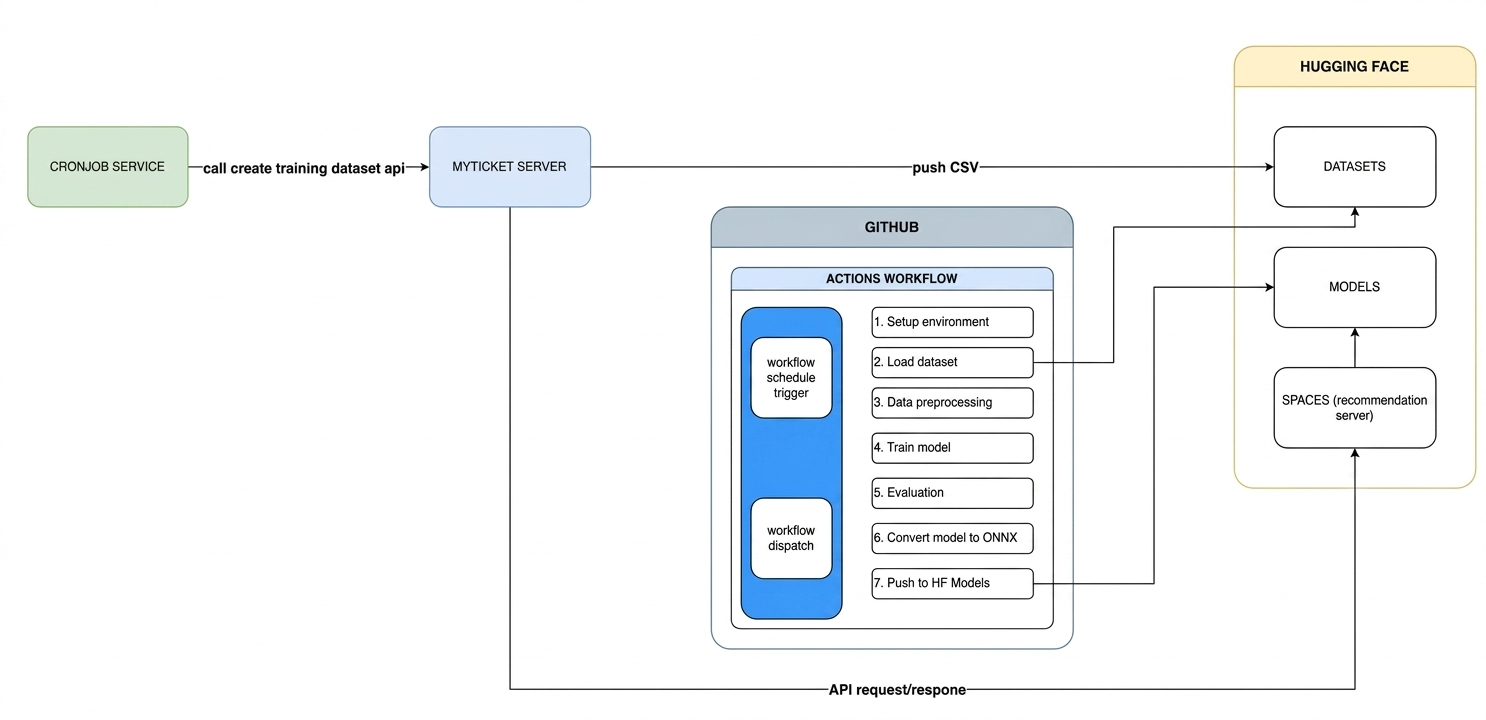
\includegraphics[width=0.9\textwidth]{Images/Quy trình xử lý hệ thống.png}
    \vspace{15pt}
    \caption{Quy trình MLOps tự động}
\end{figure}

\subsubsection{Xây dựng tập dữ liệu và Đặc trưng (Feature Engineering)}

\indent \indent \textbf{Giải pháp dữ liệu giả lập (Synthetic Data)}\\
\indent Do quy mô đồ án trong giai đoạn phát triển chưa có lượng người dùng thực tế đủ lớn, nhóm đã sử dụng AI để sinh dữ liệu giả lập. Việc này đảm bảo mô hình có đủ dữ kiện ban đầu về mối liên hệ giữa các thuộc tính người dùng và thể loại sự kiện.

\begin{table}[H]
\centering
\small
\caption{Bảng dữ liệu mẫu}
\begin{adjustbox}{width=\textwidth}
\begin{tabular}{|c|c|c|c|c|c|c|c|c|c|c|c|c|c|}
\hline
user\_id & event\_id & age & gender & avgPurchasePrice & totalSpent & totalTicketsPurchase & genre & ageLimit & eventClickCount & totalTickets & sameEventGenreClickCount & sameEventGenrePurchase & interestScore \\
\hline
4a945649c14406ab1dbf3ed5 & fa784fd8a4ef320b3500aca & 17 & 2 & 1742000 & 15678000 & 9 & 5 & 0 & 1629 & 2000 & 3 & 4 & 130 \\
\hline
4145aa00ffd2ec0f4d6ae07 & 97df4de4a6d10f463b0ce & 47 & 2 & 1773000 & 24822000 & 14 & 5 & 16 & 6477 & 500 & 14 & 4 & 130 \\
\hline
8a17f641d9a651314509a88 & b9be063d98b39a523c51ba7 & 31 & 1 & 1523000 & 28937000 & 19 & 9 & 16 & 3776 & 1000 & 4 & 1 & 130 \\
\hline
e59522f577e30a0b69a12372 & 5197e5538045bc60e0ec72c7 & 30 & 0 & 371000 & 7420000 & 20 & 6 & 16 & 7507 & 2000 & 10 & 1 & 130 \\
\hline
b4e0501d885cd68d33113b & 41e00528ea39dfada77663 & 44 & 1 & 1131000 & 15834000 & 14 & 9 & 13 & 4584 & 1000 & 9 & 0 & 130 \\
\hline
\end{tabular}
\end{adjustbox}
\end{table}
\textbf{Các nhóm đặc trưng (Features)}\\
\indent Dữ liệu huấn luyện được tổng hợp từ ba nhóm đặc trưng chính để phản ánh toàn diện mối tương quan giữa người dùng và sự kiện:
\begin{itemize}
    \item[1.] \textbf{Đặc trưng Người dùng (User Features):} Tuổi, giới tính, thói quen chi tiêu (tổng chi và giá vé trung bình đã chi).
    \item[2.] \textbf{Đặc trưng Sự kiện (Event Features):} Thể loại, giới hạn độ tuổi, quy mô (tổng số vé).
    \item[3.] \textbf{Đặc trưng Tương tác (Interaction Features):} Đây là nhóm quan trọng nhất, bao gồm số lần click vào sự kiện cụ thể, số lần click vào các sự kiện cùng thể loại và số lần mua vé các sự kiện cùng thể loại.
\end{itemize}

\indent \textbf{Nhãn dữ liệu (Labeling)}\\
\indent Để áp dụng thuật toán Ranking, biến mục tiêu interestScore được tính từ tổng hợp hành vi click và mua. Biến này được rời rạc hóa thành 5 mức độ (0 đến 4). Việc chuẩn hóa này giúp mô hình tập trung vào việc phân cấp mức độ ưu tiên thay vì dự đoán giá trị tuyệt đối.

\subsubsection{Cơ chế Lọc và Chọn Tập Ứng viên (Candidate Selection)}
\indent \indent Trước khi gửi dữ liệu đến Recommendation Server để dự đoán, hệ thống thực hiện một bước tiền xử lý nhằm xây dựng tập các sự kiện ứng viên phù hợp với từng người dùng.
\begin{itemize}
    \item[] \textbf{Bước 1 -} \textbf{Xác định thể loại yêu thích (Favorite Genres)}
    Dựa trên dữ liệu bảng Interaction, hệ thống truy xuất các sự kiện mà người dùng đã từng tương tác (click hoặc purchase), từ đó trích xuất danh sách các thể loại sự kiện tương ứng. Danh sách này được xem là tập genre yêu thích của người dùng và có thể rỗng đối với người dùng mới.

    \item[] \textbf{Bước 2 -} \textbf{Lọc danh sách sự kiện khả dụng}
    Hệ thống truy vấn tối đa 50 sự kiện thỏa mãn các điều kiện:
    \begin{itemize}
        \item[-] Trạng thái là published
        \item[-] Thời gian kết thúc (endDateTime) vẫn còn hiệu lực
        \item[-] Sắp xếp theo thời gian bắt đầu (startDateTime) theo thứ tự tăng dần (ưu tiên các sự kiện sắp diễn ra)
    \end{itemize}
    
    \item[] \textbf{Bước 3 -} \textbf{Chiến lược chọn 20 sự kiện đầu vào}
    \begin{itemize}
        \item[-] Nếu tổng số sự kiện $\le$ 20: Sử dụng toàn bộ danh sách làm đầu vào cho mô hình
        \item[-] Nếu tổng số sự kiện $>$ 20: Chia thành hai nhóm
        \begin{itemize}
            \item[+] Nhóm x: các sự kiện thuộc thể loại yêu thích
            \item[+] Nhóm y: các sự kiện còn lại
        \end{itemize}
       Việc lựa chọn tuân theo các ràng buộc:
       \begin{itemize}
            \item[1.] x $+$ y = 20
            \item[2.] x $\le$ 15
       \end{itemize}
       Hệ thống ưu tiên chọn nhiều nhất có thể từ nhóm yêu thích (tối đa 15), phần còn lại được bổ sung từ nhóm khác nhằm đảm bảo tính đa dạng (diversity) trong gợi ý.
       Trong mỗi nhóm, các sự kiện được chọn ngẫu nhiên (shuffle) để tránh thiên lệch và tăng khả năng khám phá (exploration).
    \end{itemize}
    \item[] \textbf{Bước 4 -} \textbf{Gửi đến Recommendation Server:}
    Danh sách 20 sự kiện sau khi chọn sẽ được sử dụng làm đầu vào cho mô hình học máy để tính toán điểm số và xếp hạng.\\
    \textbf{Cơ chế xử lý Cold Start}\\
    Trong giai đoạn đầu, khi dữ liệu tương tác chưa đủ lớn để huấn luyện mô hình hoặc Recommendation Server chưa sẵn sàng, hệ thống sử dụng chiến lược dự phòng:
    \begin{itemize}
        \item[-] Lấy 20 sự kiện từ danh sách đã lọc
        \item[-] Thực hiện shuffle ngẫu nhiên toàn bộ danh sách
        \item[-] Trả trực tiếp về phía Frontend mà không thông qua mô hình
    \end{itemize}
    Cách tiếp cận này giúp đảm bảo hệ thống luôn có kết quả trả về, tăng tính khám phá hành vi người dùng và thu thập thêm dữ liệu cho các lần huấn luyện sau.

\end{itemize}

\subsubsection{Thuật toán và Phương pháp huấn luyện}
\indent \indent Mô hình sử dụng thuật toán LightGBM với cấu hình LambdaRank, tập trung vào việc tối ưu thứ tự hiển thị thay vì dự đoán giá trị đơn lẻ.
\begin{itemize}
    \item[1.] \textbf{Chiến lược huấn luyện:}\\
    \textbf{Sử dụng Group K-Fold (5-fold):} dữ liệu được chia thành 5 phần (folds) dựa trên user\_id. Cách tiếp cận này đảm bảo toàn bộ hành vi của một người dùng chỉ nằm trong một tập nhất định, giúp đánh giá chính xác khả năng gợi ý cho người dùng mới mà mô hình chưa từng thấy dữ liệu tương tác.\\
    \textbf{Sử dụng Early Stopping:} tránh quá tải (overfitting) và tìm ra số vòng lặp (best\_iteration) tối ưu trước khi huấn luyện lại trên toàn bộ tập dữ liệu.
    \item[2.] \textbf{Độ đo tối ưu:} Sử dụng NDCG$@$15 (Normalized Discounted Cumulative Gain) nhằm đảm bảo các sự kiện có điểm quan tâm cao nhất luôn được đẩy lên các vị trí đầu tiên trong danh sách 15 kết quả trả về.
\end{itemize}


\subsubsection{Đánh giá và Tối ưu hóa mô hình}
\textbf{a. Độ đo xếp hạng (Ranking Metrics)}\\
\textbf{1. NDCG$@$15}\\
NDCG$@$15 được sử dụng làm độ đo chính trong quá trình huấn luyện mô hình. Độ đo này đánh giá chất lượng sắp xếp của 15 kết quả đầu tiên, đồng thời ưu tiên các sự kiện có mức độ quan tâm cao xuất hiện ở vị trí đầu danh sách.\\
\textbf{Công thức:} $DCG@K = \sum_{i=1}^{K} \frac{2^{rel_i} - 1}{\log_2(i + 1)}$ \\
\textbf{Trong đó:}
\begin{itemize}
    \item[-] $rel_i$: mức độ liên quan của sự kiện tại vị trí i (trong trường hợp của hệ thống là Relevance Level được rời rạc hoá từ interestScore)
    \item[-] $i$: vị trí của sự kiện trong danh sách gợi ý
    \item[-] $K$: số lượng kết quả được đánh giá
\end{itemize}
\textbf{Chuẩn hóa thành NDCG:} Để đưa giá trị về khoảng từ 0 đến 1, hệ thống thực hiện chuẩn hóa \\
$NDCG@K = \frac{DCG@K}{IDCG@K}$.\\
\textbf{Trong đó:} IDCG là giá trị DCG lý tưởng khi toàn bộ các sự kiện được sắp xếp hoàn hảo theo đúng mức độ quan tâm giảm dần.\\
\textbf{Ý nghĩa:}
\begin{itemize}
    \item[-] NDCG = 1 $\rightarrow$ sắp xếp hoàn hảo
    \item[-] NDCG gần 1 $\rightarrow$ thứ tự gợi ý rất tốt
    \item[-] NDCG thấp $\rightarrow$ mô hình xếp hạng chưa hiệu quả
\end{itemize}
\textbf{Kết quả thực nghiệm:} Mean NDCG$@$15 xấp xỉ 0.71\\
Giá trị này cho thấy mô hình có khả năng sắp xếp các sự kiện phù hợp lên các vị trí ưu tiên với độ chính xác tương đối cao.

\textbf{2. Precision$@$10}\\
Precision$@$10 đo tỉ lệ các sự kiện phù hợp xuất hiện trong 10 kết quả gợi ý đầu tiên.\\
\textbf{Công thức:} $Precision@K = \frac{\text{relevant items in top K}}{K}$\\
Trong top K event gợi ý, có bao nhiêu event thực sự user quan tâm.\\
\textbf{Kết quả thực nghiệm:} Mean Precision$@$10 xấp xỉ 0.84\\
Điều này cho thấy phần lớn các sự kiện được đề xuất ở top đầu đều phù hợp với sở thích và hành vi người dùng. Đây là yếu tố quan trọng trong hệ thống gợi ý vì người dùng thường chỉ quan tâm đến một số lượng nhỏ kết quả đầu tiên.

\textbf{3. MRR (Mean Reciprocal Rank)}
MRR đánh giá vị trí xuất hiện đầu tiên của một sự kiện phù hợp trong danh sách gợi ý. Nếu sự kiện phù hợp xuất hiện càng sớm thì giá trị MRR càng cao.\\
\textbf{Công thức:} $MRR = \frac{1}{|Q|} \sum_{i=1}^{|Q|} \frac{1}{rank_i}$\\
\textbf{Trong đó:} 
\begin{itemize}
    \item[-] $rank_i$ :vị trí của sự kiện phù hợp đầu tiên
    \item[-] Q: tập người dùng hoặc tập truy vấn
\end{itemize}
\textbf{Kết quả thực nghiệm:} Mean MRR xấp xỉ 0.92 \\
Kết quả này cho thấy mô hình thường đưa được ít nhất một sự kiện có mức độ quan tâm cao lên vị trí đầu tiên trong danh sách gợi ý. Điều này phản ánh khả năng ưu tiên chính xác các sự kiện phù hợp nhất đối với người dùng.\\

\textbf{b. Tính quan trọng của đặc trưng (Feature Importance)} \\
\indent Thông qua huấn luyện, mô hình xác định các đặc trưng về avgPurchasePrice, totalSpent, sameEventGenreClickCount và eventClickCount có ảnh hưởng lớn nhất đến kết quả dự đoán.
\begin{figure}[H]
    \centering
    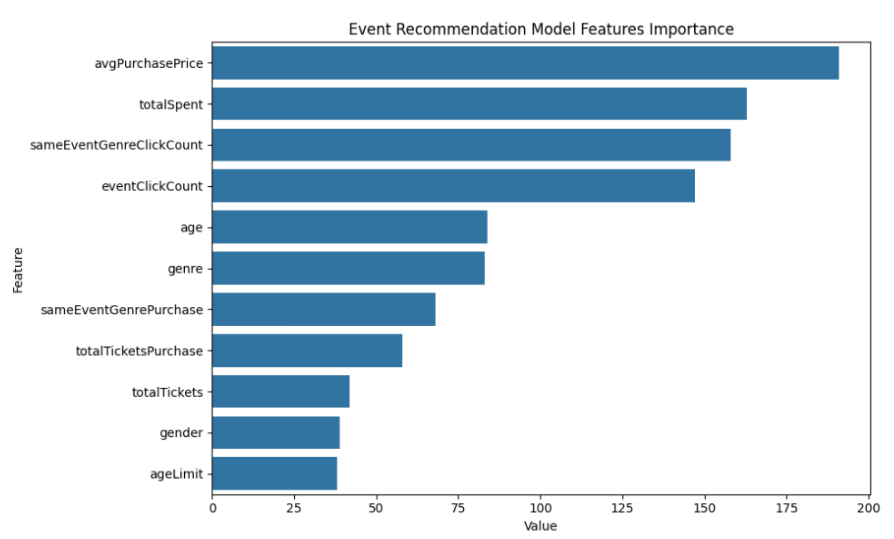
\includegraphics[width=0.6\textwidth]{Images/Các đặc trưng quan trọng mô hình gợi ý.png}
    \vspace{15pt}
    \caption{Tính quan trọng của các đặc trưng trong mô hình gợi ý}
\end{figure}
\textbf{c. Đánh giá bằng Ma trận nhầm lẫn (Confusion Matrix)}\\
\indent Để đánh giá chi tiết hiệu năng phân loại, nhóm thực hiện sử dụng ma trận nhầm lẫn trên 5 mức độ quan tâm (từ 0 đến 4).
\begin{figure}[H]
    \centering
    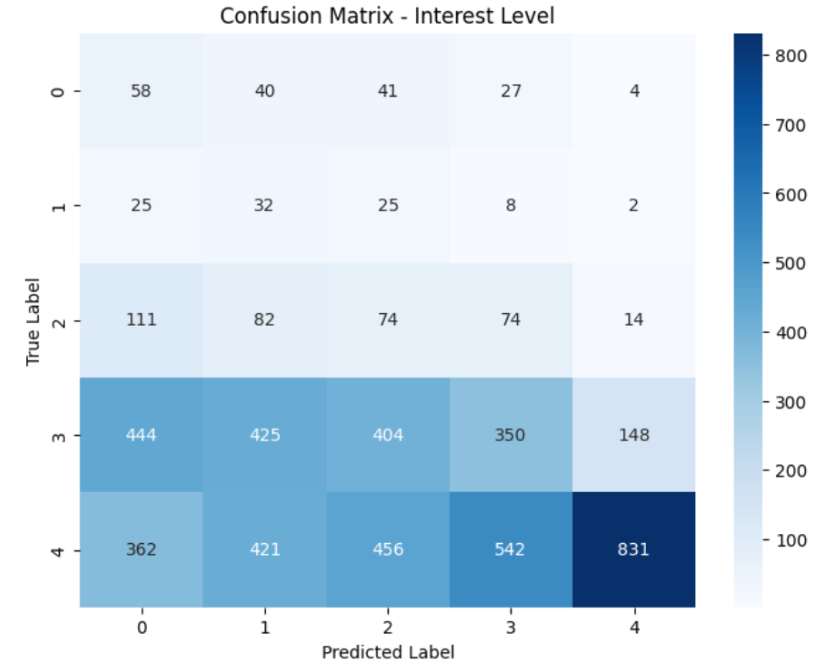
\includegraphics[width=0.6\textwidth]{Images/Confusion matrix.png}
    \vspace{15pt}
    \caption{Ma trận nhầm lẫn của mô hình gợi ý}
\end{figure}
\begin{itemize}
    \item[-] \textbf{Kết quả:} Mô hình thể hiện khả năng phân loại vượt trội ở các nhãn cực đoan (Nhãn 0 - Không quan tâm và Nhãn 4 - Rất quan tâm). Điều này chứng minh thuật toán LambdaRank hoạt động hiệu quả trong việc phân tách rõ rệt các đối tượng mục tiêu.
    \item[-] \textbf{Phân tích sai số:} Một số sự nhầm lẫn xảy ra giữa các nhãn kề nhau (ví dụ: nhãn 2 và 3). Điều này là hợp lý trong bài toán gợi ý, vì ranh giới định lượng giữa các mức độ "quan tâm trung bình" thường có sự giao thoa lớn, không ảnh hưởng quá nhiều đến trải nghiệm xếp hạng tổng thể.
\end{itemize}

\textbf{d. Tối ưu hóa với định dạng ONNX}\\
\indent Để đưa mô hình vào vận hành thực tế, nhóm đã thực hiện chuyển đổi định dạng sang ONNX (Open Neural Network Exchange). Giải pháp này mang lại hai lợi ích cốt lõi:
\begin{itemize}
    \item[-] \textbf{Tối ưu hiệu năng:} Giảm đáng kể độ trễ khi dự đoán (Inference Latency), cho phép Recommendation Server phản hồi danh sách gợi ý gần như tức thời khi nhận yêu cầu từ Web Server.
    \item[-] \textbf{Tính độc lập:} Loại bỏ sự phụ thuộc vào thư viện huấn luyện gốc (LightGBM) trong môi trường production, giúp hệ thống gọn nhẹ, dễ dàng mở rộng và tương thích tốt với nhiều nền tảng phần cứng khác nhau.
\end{itemize}

\subsubsection{Đánh giá hiệu năng hệ thống MLOps}
\textbf{a. inference latency}\\
Inference Latency là độ trễ từ thời điểm Recommendation Server nhận yêu cầu cho đến khi trả về kết quả gợi ý.\\
Để đánh giá khả năng phản hồi của hệ thống trong môi trường thực tế, nhóm sử dụng công cụ kiểm thử tải k6 để gửi đồng thời nhiều request đến Recommendation Server được triển khai trên Hugging Face Spaces.\\
%chèn bảng
\textbf{Kết quả:}
\begin{itemize}
    \item[-] Hệ thống duy trì độ trễ trung bình dưới 350 ms ngay cả khi xử lý đồng thời 100 người dùng kéo dài trong khoảng 30s.
    \item[-] Tỉ lệ lỗi bằng 0\% trong toàn bộ quá trình kiểm thử ở mức tải thông thường.
    \item[-] Recommendation Server có khả năng phục vụ realtime inference tương đối ổn định cho hệ thống gợi ý sự kiện.
\end{itemize}
Nhóm tiếp tục thử nghiệm ở mức tải cực lớn (1000 VUs). Khi đó hệ thống xuất hiện cơ chế rate limiting từ Hugging Face Spaces:\\
%chèn bảng
Nguyên nhân không đến từ lỗi mô hình mà do nền tảng Hugging Face Spaces giới hạn lưu lượng truy cập nhằm bảo vệ tài nguyên hệ thống. Điều này cho thấy Recommendation Server vẫn có khả năng xử lý tải lớn nhưng bị giới hạn bởi hạ tầng triển khai miễn phí.\\
\textbf{b. Training time}\\
Trong quá trình thực nghiệm, thời gian huấn luyện toàn bộ mô hình LightGBM LambdaRank trên tập dữ liệu hiện tại đạt khoảng 0.037 giây. Kết quả này cho thấy mô hình có tốc độ huấn luyện rất nhanh nhờ vào các đặc điểm:
\begin{itemize}
    \item[-] Thuật toán LightGBM được tối ưu cho dữ liệu dạng bảng (tabular data).
    \item[-] Kích thước đặc trưng đầu vào tương đối nhỏ.
    \item[-] Quá trình huấn luyện sử dụng cơ chế Early Stopping giúp giảm số vòng lặp không cần thiết.
    \item[-] Hạ tầng GitHub Actions hỗ trợ tự động hóa pipeline MLOps mà không cần can thiệp thủ công.
\end{itemize}
Thời gian huấn luyện thấp mang lại lợi thế lớn cho hệ thống MLOps, cho phép mô hình được cập nhật thường xuyên khi có dữ liệu tương tác mới từ người dùng mà vẫn đảm bảo chi phí vận hành thấp và tốc độ triển khai nhanh.\\
\textbf{c. Model size}\\
Sau khi huấn luyện, mô hình được lưu dưới hai định dạng khác nhau:\\
%chèn bảng
Kết quả cho thấy phiên bản ONNX có kích thước nhỏ hơn so với mô hình LightGBM gốc. Điều này giúp:
\begin{itemize}
    \item[-] Giảm dung lượng lưu trữ trên hệ thống triển khai.
    \item[-] Tăng tốc độ tải mô hình khi Recommendation Server khởi động.
    \item[-] Giảm băng thông khi tự động cập nhật mô hình từ Hugging Face Models.
    \item[-] Tối ưu hiệu năng inference trong môi trường production.
\end{itemize}
Ngoài ra, việc chuyển đổi sang định dạng ONNX còn giúp mô hình độc lập với thư viện huấn luyện gốc, tăng khả năng tương thích và mở rộng trên nhiều nền tảng triển khai khác nhau.

\subsubsection{Kết luận và Hướng phát triển}
\indent \indent \textbf{Kết quả:} Xây dựng thành công pipeline tự động từ khâu dữ liệu đến triển khai, đáp ứng bài toán gợi ý thực tế với độ trễ thấp.\\
\indent \textbf{Hướng cải thiện:} Tích hợp thêm các kỹ thuật xử lý ngôn ngữ tự nhiên (NLP) để phân tích mô tả sự kiện sâu hơn cũng như phân tích hình ảnh banner sự kiện để tăng độ chính xác của gợi ý.

\subsection{Quy trình xuất dữ liệu Danh sách khách hàng (PDF/CSV)}
Chức năng xuất dữ liệu Danh sách khách hàng (PDF/CSV) được thiết kế dành riêng cho vai trò Organizer (Ban tổ chức), 
cho phép trích xuất dữ liệu danh sách các khách hàng đã thanh toán thành công vé của một sự kiện cụ thể, tạo tiền đề để phát triển thêm các chức năng mới về sau như đối soát, 
chăm sóc khách hàng và vận hành check-in tại sự kiện. 
Giải pháp hướng đến việc giảm tải cho server bằng cách đẩy việc sinh tệp (render file) về phía Client (Frontend) sau khi nhận được dataset chuẩn hóa từ Backend.\\
\textbf{Quy trình được thực hiện qua 3 giai đoạn chính:}
\begin{itemize}
    \item[1.] \textbf{Truy vấn và Tổng hợp (Backend)}
    \begin{itemize}
        \item[-] Hệ thống xác thực quyền sở hữu sự kiện thông qua Middleware JWT và kiểm tra quan hệ giữa Organizer với Event.
        \item[-] Thực hiện truy vấn liên kết (Aggregation) giữa các tập thực thể: Purchase (trạng thái "paid"), User, TicketClass và Ticket.
        \item[-] Logic xử lý quan trọng: Backend không trả về dữ liệu thô mà thực hiện "làm phẳng" (Flattening) dữ liệu thành một mảng JSON attendeeRows duy nhất để Frontend dễ dàng xử lý mà không cần tính toán lại logic nghiệp vụ.
    \end{itemize}
    \item[2.] \textbf{Chuẩn hóa hiển thị (Frontend)}
    \begin{itemize}
        \item[-] Dữ liệu sau khi nhận được từ API được map thành các interface TypeScript (AttendeeRow) để đảm bảo tính nhất quán.
        \item[-] Các trường thông tin (tên, giá vé, thời gian mua) được format theo quy chuẩn địa phương (vi-VN) và sắp xếp theo tên khách hàng trước khi đưa vào bảng hiển thị.
    \end{itemize}
    \item[3.] \textbf{Kích hoạt Export}
    \begin{itemize}
        \item[-] Đối với CSV: Sử dụng Blob API để tạo tệp trực tiếp từ chuỗi text. Đặc biệt, hệ thống thêm ký tự BOM ($uFEFF$) để đảm bảo file hiển thị đúng định dạng tiếng Việt khi mở bằng Excel.
        \item[-] Đối với PDF: Sử dụng thư viện jsPDF kết hợp plugin jspdf-autotable. Dữ liệu được vẽ lên canvas theo khổ ngang (A4 Landscape) để tối ưu không gian hiển thị cho bảng nhiều cột thông tin.
    \end{itemize}
\end{itemize}
\textbf{Các kỹ thuật đặc trưng:}
\begin{itemize}
    \item[-] \textbf{Xác thực:} Đảm bảo tính an toàn dữ liệu khách hàng thông qua kiểm tra chéo giữa organizerId và req.user.id.
    \item[-] \textbf{Hiệu suất:} Việc sử dụng Frontend để tạo file giúp hệ thống không phải lưu trữ tệp tạm trên máy chủ, tối ưu tài nguyên lưu trữ.
\end{itemize}
\begin{figure}[H]
    \centering
    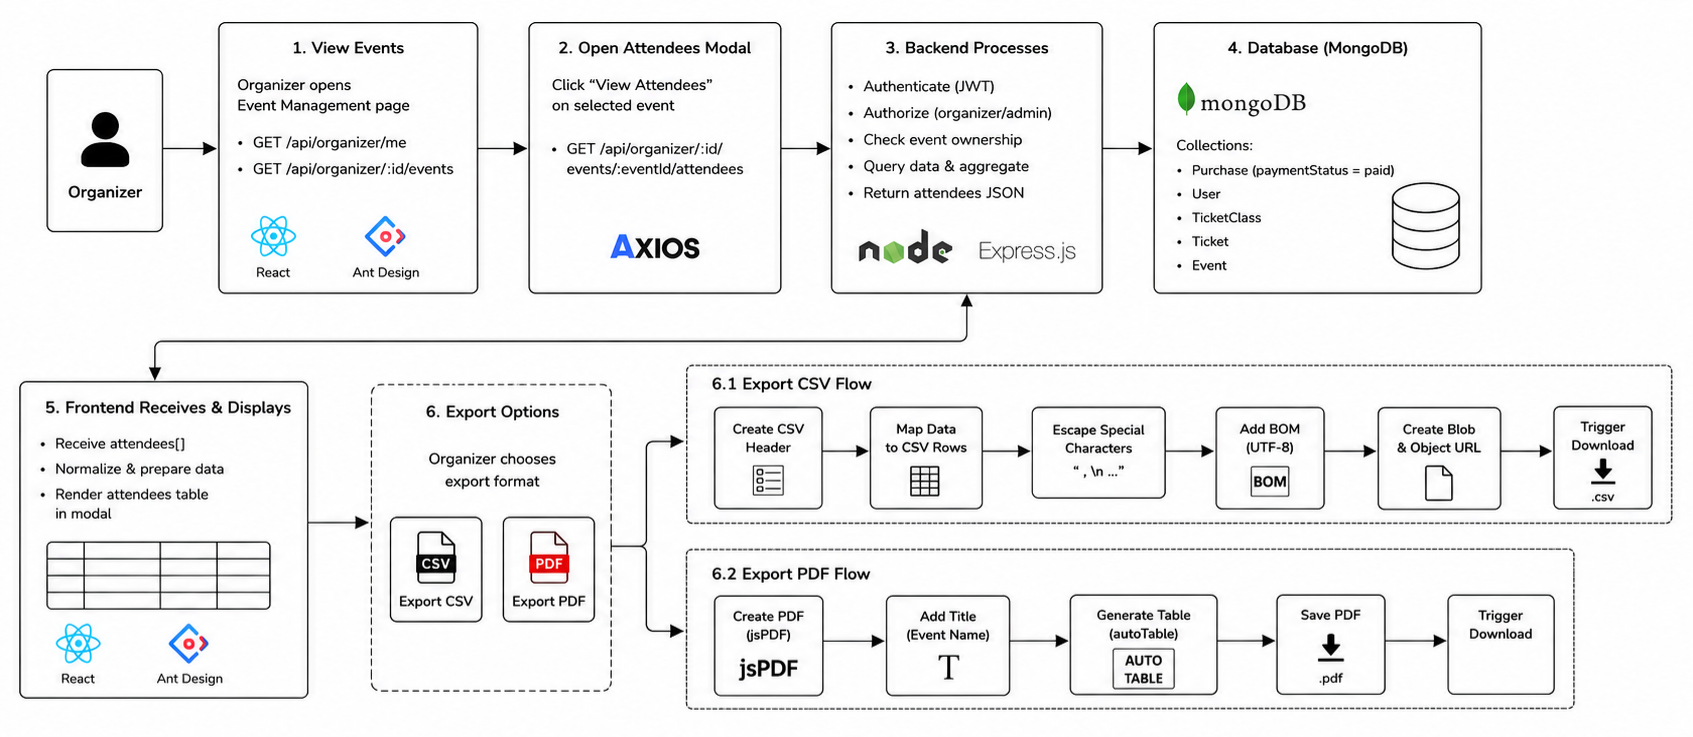
\includegraphics[width=1\textwidth]{Images/Cơ chế xuất file.png}
    \vspace{15pt}
    \caption{Quy trình xuất dữ liệu Danh sách khách hàng}
\end{figure}

\subsection{Cơ chế quản lý Mã QR và Vé điện tử}
Hệ thống áp dụng phương pháp "Public URL Encoding": Mã QR không chứa dữ liệu vé thô mà chứa một liên kết công khai dẫn tới trang thông tin vé điện tử (/ticket-info/:ticketId).\\
\textbf{Mục tiêu hướng tới:}
\begin{itemize}
    \item[-] Mã QR đơn giản, dễ quét ngay cả ở độ phân giải thấp.
    \item[-] Có thể cập nhật giao diện hiển thị hoặc bổ sung thông tin vé mà không cần thu hồi/đổi mã QR đã phát hành.
    \item[-] Dễ dàng tích hợp đa kênh (Web preview, Email, Tải ảnh).
\end{itemize}
\textbf{Quy trình xử lý đa luồng:}
\begin{itemize}
    \item[a.] \textbf{Luồng hiển thị và Tải xuống (Client-side)}
    \begin{itemize}
        \item[-] \textbf{Xem nhanh (Preview):} Khi người dùng mở lịch sử vé, Frontend sử dụng component QRCode của Ant Design để vẽ mã QR ngay lập tức từ dữ liệu sẵn có, giúp phản hồi giao diện đạt tốc độ tối đa (Real-time).
        \item[-] \textbf{Tải xuống (Server-side):} Khi có yêu cầu lưu tệp, hệ thống gọi API GET /.../qr-image. Backend sử dụng thư viện qrcode để sinh một Buffer ảnh PNG chuẩn, hỗ trợ lưu trữ lâu dài trên thiết bị người dùng.
    \end{itemize}
    \item[b.] \textbf{Luồng Email xác nhận (Automated Trigger)}\\
    Sau khi thanh toán thành công (hoặc đơn hàng 0đ được xác nhận), hệ thống kích hoạt luồng gửi email tự động qua SendGrid:
    \begin{itemize}
        \item[1.] \textbf{Tạo Attachment:} Mỗi vé trong đơn hàng được sinh một ảnh QR riêng biệt dưới dạng Buffer.
        \item[2.] \textbf{Nhúng Inline (CID):} Để tránh việc ảnh bị chặn bởi các trình duyệt mail (như Gmail/Outlook), hệ thống sử dụng cơ chế nhúng cid. Ảnh QR sẽ xuất hiện trực tiếp trong nội dung HTML của email thay vì chỉ là tệp đính kèm rời rạc.
    \end{itemize}
    \item[c.] \textbf{Quy trình quét và Xác thực (Validation)}\\
    Khi nhân viên check-in quét mã QR (hoặc người dùng bấm link email):
    \begin{itemize}
        \item[1.] Frontend điều hướng tới route TicketInfoPage dựa trên ID trong mã QR.
        \item[2.] Hệ thống gọi Public API để lấy thông tin chi tiết (Tên sự kiện, Loại vé, Vị trí ghế).
        \item[3.] Kiểm tra tính hợp lệ: Backend kiểm tra trạng thái thanh toán (paymentStatus = paid) trước khi trả về dữ liệu, đảm bảo chỉ những vé hợp lệ mới được hiển thị thông tin.
    \end{itemize}
\end{itemize}
\begin{figure}[H]
    \centering
    \includegraphics[width=1\textwidth]{Images/Cơ chế QR code.png}
    \vspace{15pt}
    \caption{Cơ chế quản lý Mã QR và Vé điện tử}
\end{figure}

